% Options for packages loaded elsewhere
\PassOptionsToPackage{unicode}{hyperref}
\PassOptionsToPackage{hyphens}{url}
%
\documentclass[
  a4paper,
]{scrbook}

\usepackage{amsmath,amssymb}
\usepackage[]{gfsartemisia}
\usepackage{iftex}
\ifPDFTeX
  \usepackage[T1]{fontenc}
  \usepackage[utf8]{inputenc}
  \usepackage{textcomp} % provide euro and other symbols
\else % if luatex or xetex
  \usepackage{unicode-math}
  \defaultfontfeatures{Scale=MatchLowercase}
  \defaultfontfeatures[\rmfamily]{Ligatures=TeX,Scale=1}
\fi
% Use upquote if available, for straight quotes in verbatim environments
\IfFileExists{upquote.sty}{\usepackage{upquote}}{}
\IfFileExists{microtype.sty}{% use microtype if available
  \usepackage[]{microtype}
  \UseMicrotypeSet[protrusion]{basicmath} % disable protrusion for tt fonts
}{}
\makeatletter
\@ifundefined{KOMAClassName}{% if non-KOMA class
  \IfFileExists{parskip.sty}{%
    \usepackage{parskip}
  }{% else
    \setlength{\parindent}{0pt}
    \setlength{\parskip}{6pt plus 2pt minus 1pt}}
}{% if KOMA class
  \KOMAoptions{parskip=half}}
\makeatother
\usepackage{xcolor}
\usepackage[margin = 2.5cm]{geometry}
\setlength{\emergencystretch}{3em} % prevent overfull lines
\setcounter{secnumdepth}{5}
% Make \paragraph and \subparagraph free-standing
\ifx\paragraph\undefined\else
  \let\oldparagraph\paragraph
  \renewcommand{\paragraph}[1]{\oldparagraph{#1}\mbox{}}
\fi
\ifx\subparagraph\undefined\else
  \let\oldsubparagraph\subparagraph
  \renewcommand{\subparagraph}[1]{\oldsubparagraph{#1}\mbox{}}
\fi
\pagestyle{headings}

\usepackage{color}
\usepackage{fancyvrb}
\newcommand{\VerbBar}{|}
\newcommand{\VERB}{\Verb[commandchars=\\\{\}]}
\DefineVerbatimEnvironment{Highlighting}{Verbatim}{commandchars=\\\{\}}
% Add ',fontsize=\small' for more characters per line
\newenvironment{Shaded}{}{}
\newcommand{\AlertTok}[1]{\textcolor[rgb]{1.00,0.33,0.33}{\textbf{#1}}}
\newcommand{\AnnotationTok}[1]{\textcolor[rgb]{0.42,0.45,0.49}{#1}}
\newcommand{\AttributeTok}[1]{\textcolor[rgb]{0.84,0.23,0.29}{#1}}
\newcommand{\BaseNTok}[1]{\textcolor[rgb]{0.00,0.36,0.77}{#1}}
\newcommand{\BuiltInTok}[1]{\textcolor[rgb]{0.84,0.23,0.29}{#1}}
\newcommand{\CharTok}[1]{\textcolor[rgb]{0.01,0.18,0.38}{#1}}
\newcommand{\CommentTok}[1]{\textcolor[rgb]{0.42,0.45,0.49}{#1}}
\newcommand{\CommentVarTok}[1]{\textcolor[rgb]{0.42,0.45,0.49}{#1}}
\newcommand{\ConstantTok}[1]{\textcolor[rgb]{0.00,0.36,0.77}{#1}}
\newcommand{\ControlFlowTok}[1]{\textcolor[rgb]{0.84,0.23,0.29}{#1}}
\newcommand{\DataTypeTok}[1]{\textcolor[rgb]{0.84,0.23,0.29}{#1}}
\newcommand{\DecValTok}[1]{\textcolor[rgb]{0.00,0.36,0.77}{#1}}
\newcommand{\DocumentationTok}[1]{\textcolor[rgb]{0.42,0.45,0.49}{#1}}
\newcommand{\ErrorTok}[1]{\textcolor[rgb]{1.00,0.33,0.33}{\underline{#1}}}
\newcommand{\ExtensionTok}[1]{\textcolor[rgb]{0.84,0.23,0.29}{\textbf{#1}}}
\newcommand{\FloatTok}[1]{\textcolor[rgb]{0.00,0.36,0.77}{#1}}
\newcommand{\FunctionTok}[1]{\textcolor[rgb]{0.44,0.26,0.76}{#1}}
\newcommand{\ImportTok}[1]{\textcolor[rgb]{0.01,0.18,0.38}{#1}}
\newcommand{\InformationTok}[1]{\textcolor[rgb]{0.42,0.45,0.49}{#1}}
\newcommand{\KeywordTok}[1]{\textcolor[rgb]{0.84,0.23,0.29}{#1}}
\newcommand{\NormalTok}[1]{\textcolor[rgb]{0.14,0.16,0.18}{#1}}
\newcommand{\OperatorTok}[1]{\textcolor[rgb]{0.14,0.16,0.18}{#1}}
\newcommand{\OtherTok}[1]{\textcolor[rgb]{0.44,0.26,0.76}{#1}}
\newcommand{\PreprocessorTok}[1]{\textcolor[rgb]{0.84,0.23,0.29}{#1}}
\newcommand{\RegionMarkerTok}[1]{\textcolor[rgb]{0.42,0.45,0.49}{#1}}
\newcommand{\SpecialCharTok}[1]{\textcolor[rgb]{0.00,0.36,0.77}{#1}}
\newcommand{\SpecialStringTok}[1]{\textcolor[rgb]{0.01,0.18,0.38}{#1}}
\newcommand{\StringTok}[1]{\textcolor[rgb]{0.01,0.18,0.38}{#1}}
\newcommand{\VariableTok}[1]{\textcolor[rgb]{0.89,0.38,0.04}{#1}}
\newcommand{\VerbatimStringTok}[1]{\textcolor[rgb]{0.01,0.18,0.38}{#1}}
\newcommand{\WarningTok}[1]{\textcolor[rgb]{1.00,0.33,0.33}{#1}}

\providecommand{\tightlist}{%
  \setlength{\itemsep}{0pt}\setlength{\parskip}{0pt}}\usepackage{longtable,booktabs,array}
\usepackage{calc} % for calculating minipage widths
% Correct order of tables after \paragraph or \subparagraph
\usepackage{etoolbox}
\makeatletter
\patchcmd\longtable{\par}{\if@noskipsec\mbox{}\fi\par}{}{}
\makeatother
% Allow footnotes in longtable head/foot
\IfFileExists{footnotehyper.sty}{\usepackage{footnotehyper}}{\usepackage{footnote}}
\makesavenoteenv{longtable}
\usepackage{graphicx}
\makeatletter
\def\maxwidth{\ifdim\Gin@nat@width>\linewidth\linewidth\else\Gin@nat@width\fi}
\def\maxheight{\ifdim\Gin@nat@height>\textheight\textheight\else\Gin@nat@height\fi}
\makeatother
% Scale images if necessary, so that they will not overflow the page
% margins by default, and it is still possible to overwrite the defaults
% using explicit options in \includegraphics[width, height, ...]{}
\setkeys{Gin}{width=\maxwidth,height=\maxheight,keepaspectratio}
% Set default figure placement to htbp
\makeatletter
\def\fps@figure{htbp}
\makeatother
\newlength{\cslhangindent}
\setlength{\cslhangindent}{1.5em}
\newlength{\csllabelwidth}
\setlength{\csllabelwidth}{3em}
\newlength{\cslentryspacingunit} % times entry-spacing
\setlength{\cslentryspacingunit}{\parskip}
\newenvironment{CSLReferences}[2] % #1 hanging-ident, #2 entry spacing
 {% don't indent paragraphs
  \setlength{\parindent}{0pt}
  % turn on hanging indent if param 1 is 1
  \ifodd #1
  \let\oldpar\par
  \def\par{\hangindent=\cslhangindent\oldpar}
  \fi
  % set entry spacing
  \setlength{\parskip}{#2\cslentryspacingunit}
 }%
 {}
\usepackage{calc}
\newcommand{\CSLBlock}[1]{#1\hfill\break}
\newcommand{\CSLLeftMargin}[1]{\parbox[t]{\csllabelwidth}{#1}}
\newcommand{\CSLRightInline}[1]{\parbox[t]{\linewidth - \csllabelwidth}{#1}\break}
\newcommand{\CSLIndent}[1]{\hspace{\cslhangindent}#1}

\usepackage{titling}
\setlength{\droptitle}{-3cm}
\preauthor{
  \begin{center}
  
\includegraphics[width=5in,height=4in]{cover.png}\\ % cover figure
  \Large
  \vspace{10mm}
}
\postauthor{
  \end{center}
}
\predate{
  \begin{center}
  Collège International des Scicences Territoriales \\ 
  Encadré par Hugues Pécout - Ingénieur de recherche, géomaticien\\
  \vspace{5mm}
  Master Carthagéo\\
  \vspace{5mm}
}
\postdate{
  \vspace{10mm}
  \\
  
\includegraphics[width=4in,height=1in]{figures/logos/logos3.jpg}\\
  % 
\includegraphics[width=1.5in,height=1.5in]{figures/logos/logos.jpg}\\
  \end{center}
  \newpage
  \mbox{}
  \vfill
  % Cover page\\
  % \emph{Beckwithia glacialis} on Snøhetta.
 }
\makeatletter
\makeatother
\makeatletter
\@ifpackageloaded{caption}{}{\usepackage{caption}}
\AtBeginDocument{%
\ifdefined\contentsname
  \renewcommand*\contentsname{Table of contents}
\else
  \newcommand\contentsname{Table of contents}
\fi
\ifdefined\listfigurename
  \renewcommand*\listfigurename{List of Figures}
\else
  \newcommand\listfigurename{List of Figures}
\fi
\ifdefined\listtablename
  \renewcommand*\listtablename{List of Tables}
\else
  \newcommand\listtablename{List of Tables}
\fi
\ifdefined\figurename
  \renewcommand*\figurename{Figure}
\else
  \newcommand\figurename{Figure}
\fi
\ifdefined\tablename
  \renewcommand*\tablename{Table}
\else
  \newcommand\tablename{Table}
\fi
}
\@ifpackageloaded{float}{}{\usepackage{float}}
\floatstyle{ruled}
\@ifundefined{c@chapter}{\newfloat{codelisting}{h}{lop}}{\newfloat{codelisting}{h}{lop}[chapter]}
\floatname{codelisting}{Listing}
\newcommand*\listoflistings{\listof{codelisting}{List of Listings}}
\makeatother
\makeatletter
\@ifpackageloaded{caption}{}{\usepackage{caption}}
\@ifpackageloaded{subcaption}{}{\usepackage{subcaption}}
\makeatother
\makeatletter
\@ifpackageloaded{tcolorbox}{}{\usepackage[many]{tcolorbox}}
\makeatother
\makeatletter
\@ifundefined{shadecolor}{\definecolor{shadecolor}{rgb}{.97, .97, .97}}
\makeatother
\makeatletter
\makeatother
\ifLuaTeX
  \usepackage{selnolig}  % disable illegal ligatures
\fi
\IfFileExists{bookmark.sty}{\usepackage{bookmark}}{\usepackage{hyperref}}
\IfFileExists{xurl.sty}{\usepackage{xurl}}{} % add URL line breaks if available
\urlstyle{same} % disable monospaced font for URLs
\hypersetup{
  pdftitle={Gestion d'une base de données qualitative et géometrique},
  pdfauthor={Elina Marveaux},
  hidelinks,
  pdfcreator={LaTeX via pandoc}}

\title{Gestion d'une base de données qualitative et géometrique}
\author{Elina Marveaux}
\date{12-06-2022}

\begin{document}
\frontmatter
\maketitle
Résumé

Résumé du stage (dont le sujet) en 10 lignes en français et en anglais.
Informatif et concis, ce résumé doit refléter l'esprit du document, définir les buts et les méthodes,
les résultats et les conclusions. Il se présente sous la forme d'un paragraphe unique, sans alinéa.

\ifdefined\Shaded\renewenvironment{Shaded}{\begin{tcolorbox}[boxrule=0pt, borderline west={3pt}{0pt}{shadecolor}, frame hidden, enhanced, interior hidden, sharp corners, breakable]}{\end{tcolorbox}}\fi

\renewcommand*\contentsname{Table des matières}
{
\setcounter{tocdepth}{2}
\tableofcontents
}
\mainmatter
\hypertarget{introduction}{%
\chapter{Introduction}\label{introduction}}

Elle doit mentionner : les objectifs, les lieux d'étude, l'intérêt du
projet : pour un public particulier ? Une nouvelle méthodologie ? Une
monographie sur un espace donné ? Durée. Un rapport orienté « recherche
» développera la problématique qui sous-tend le questionnement de
recherche et formulera, le cas échéant, les hypothèses de travail.

\hypertarget{notes-rendez-vous-antoine}{%
\chapter{Notes rendez-vous Antoine}\label{notes-rendez-vous-antoine}}

Dimension politique des visualisation à mettre en avant

\hypertarget{les-visualisations}{%
\section{Les visualisations}\label{les-visualisations}}

Faire la différences entres les visualisations des polygone sen internes
pour leur diagnostique et la présentation des ``problèmes'' et la
représentation finale, les cartographies qui doivent être finie et
présentées comme résultat et non pas comme exploration.\\
Les deux modes de représentations font appels à des enjeux différents
(ainsi que des publiques, objectifs)

\hypertarget{muxe9thodologie}{%
\section{Méthodologie}\label{muxe9thodologie}}

\begin{itemize}
\tightlist
\item
  Décrire la méthodologie
\item
  Quelle est la qualité de l'information :
\item
  Qualité du point de vue de la géomatique
\item
  Quels biais introduits dans les enquêtes ``habituelles'' ou en tout
  cas celle précédent celle-ci (eurobroadmap)
\item
  Quel biais introduits par la méthodologie actuelle, quel enjeux vis à
  vis du choix de l'outil
\item
  Comment sont identifiés/détectés les problèmes dans la BD et BDG,
  quelles propositions sont avancées , lesquelles sont mises en place et
  comment trancher ? **proposer une chaîne de traitement sous forme
  d'image''
\item
  Voir Lena Sanders : modèle LOgit pour explorer la significativité ou
  non du univ\_field
\item
  Quelle pondération de polygones lorsqu'ils se superposent, lorsqu'ils
  n'ont pas la même taille mais décrivent des ensembles similaires
  (pays) ou lorsqu'il sont multi-polygones donc séparés et parfois se
  recouvrent
\item
  Comment analyser les aires disjointes ou emboîtées ?
\end{itemize}

\hypertarget{analyse-du-besoin-en-amont}{%
\section{Analyse du besoin en amont
?}\label{analyse-du-besoin-en-amont}}

\hypertarget{livrables}{%
\section{Livrables}\label{livrables}}

\begin{itemize}
\tightlist
\item
  Quels sont les produits à réalisés et à qui s'adressent-ils ?
\item
  Priorité sur les \textbf{géométries} et leur enjeux :
\item
  plusieurs dessins sont autorisées
\item
  plusieurs modes de saisi sont possibles chacun avec leur biais
\item
  Plusieurs problèmes en découlent
\item
  Base de donnée Géo et Respondent avec documents de présentation
\item
  explorations de la BDG :
\item
  Visualisations exploratoires et travail de représentation pour le
  diagnostic (explorer les chorèmes pour proposer une typologie des
  polygones et relations rencontrées dans la BDG)
\item
  Visualisations finales / exploratoires en tant de résultats de
  l'exploration : on parle de représentations visant à proposer
  certaines interprétations des résultats (sous formes de prototypes car
  la valorisation finale est attendue en dehors du cadre du stage)
\end{itemize}

\hypertarget{git}{%
\section{GIT}\label{git}}

\begin{itemize}
\tightlist
\item
  expliquer l'intérêt de l'outil
\item
  Faire la différence entre 'usage généraliste de l'outil et l'usage
  qu'on en fait en interne (dans le care du stage notamment)
\item
  Expliquer pourquoi une page web et quel est l'intérêt (éventuellement
  pour mettre à disposition des résultats du stage et la présentation du
  mémoire ar exemple)
\end{itemize}

\hypertarget{gestion-de-projet-workshop}{%
\section{Gestion de projet /
Workshop}\label{gestion-de-projet-workshop}}

Ici discuter des apports du stage dans le domaine de la gestion de
projet et de la mise en place d'un workshop. - Dans quelle mesure
suis-je force de proposition - Quel suivi, même informel est mis ou
ai-je mis en place ? Finalement le suivi est assez souple, je suis libre
de faire ce que je veux mais le cadre est bien posé et les objectifs
déterminés. Par exemple, j'ai été accompagnée dans la découverte de la
BD e des premiers scripts exploratoires, j'ai eu comme objectif de
réaliser un document de présentation de cette base de donnée et des
traitements qui y ont été réalisés pour la rendre propre ou qui peuvent
être réalisés dessus en guise d'exploration. J'ai le champ libre pour la
réalisation de ce document concernant à la fois les outils que j'utilise
et ce que j'y met. Je reste encadrée lorsque j'ai des questions et ait
besoin d'être recadrée.

\begin{itemize}
\tightlist
\item
  Mettre ne avant l'informel : les formations et les autres projets/
  présentations auxquelles j'ai été invitées à participer
\item
  Parler des compétences acquises en matière de logiciels/ technique
  (quarto, redaction latex/yaml, regex, git )
\end{itemize}

\hypertarget{traitement-de-la-base-de-donnuxe9e-guxe9omuxe9tries}{%
\section{Traitement de la base de donnée
``géométries''}\label{traitement-de-la-base-de-donnuxe9e-guxe9omuxe9tries}}

Possibilité de créer un package pour exploiter les données.\\
Pour produire des tableaux à la volée (BDG \& BDR) et les gaphiques,
cartes, statistiques qui en découlent. Ce travail necessite
l'identification précise de productions pour chacun de ces volets (quels
graphiques sur quelles données, etc).

\hypertarget{guxe9omuxe9tries-et-leur-classification-pistes}{%
\subsection{Géométries et leur classification :
pistes}\label{guxe9omuxe9tries-et-leur-classification-pistes}}

\begin{itemize}
\tightlist
\item
  Comparer la superficie du polygone avec la superficie réelle de
  l'espace décrit (notamment lorsque le mot attribué correspond à cet
  espace).
\item
  Quel ordre des polygones pour un meme mot donnée
\item
  Justifier l'usage des menus e leur pertinences vis à vis d'une
  approche automatisée.

  \begin{itemize}
  \tightlist
  \item
    Geom repair : intersection
  \item
    txt move/add : au cas ou mais tres peu utilisé finalement
  \item
    Typologie : difficle de faire une typologie automatisée (on peut
    imaginer un scale comme etant une hierarchie des superficie
    lorsqu'elles sont contenues les unes dans les autres à x\%, mais le
    multi unique et le overlap sont plus complexes car relevent d'une
    appréciation de l'intention du dessinateur (l'intersection partielle
    de deux ensemble peut etre due à une imprecision comme à une volonté
    du dessinateur))
  \end{itemize}
\end{itemize}

\hypertarget{la-visualisation-pour-exploration}{%
\subsection{La visualisation pour
exploration}\label{la-visualisation-pour-exploration}}

\textbf{\emph{Décrire la méthode d'affichage et de classificationd es
polygones puis exposer les problèmes}} \textbf{\emph{Présenter les
problèmes de géométrie sous forme de shémas / chorème ?}}

Problème sémiolgiques pour juger rapidement et efficacement dans un
premier temps du polygone, puis dans un second temps des choix fait sur
ce/ces polygones (controle).

Le choix du fond de carte et de sa généralisation posent des enjeux
concernant d'une part les polygones décrivant des territoires insulaires
qui n'apparaissent pas et d'autre part des polygones décrivant des
petits territoires type villes dont on ne peut distinguer les contours.

Dans le premier cas, on visualise un polygone dans un océan sans repères
autour (pas d'iles), on peut estimer la justesse du dessin grace aux
informations récupérées directement du répondant (le mot associé ou son
université d'appartenance surtout) ainsi que par les autres polygones
dessinée (lorsqu'il y en a). Surtout ce problème est corrigé en
choisissant une echelle de représentation plus fine pour le fond de
carte.

Dans le second cas le problème est plus délicat. Il ne s'agit pas d'une
niveau de détail du à la généralisation mais à des limites
adminstratives ou de toponymes présents ou non pour aider à reconaitre
le lieu décrit par le polygone Dans ce cas, choisir un fond de carte
plus riche pose d'abord la contrainte de l'alourdissement de la
représentation, de la saturation de l'espace visuel au détriment du
jugement du polygone (qui est l'objet premier necessitant toute
l'attention du visualisateur). Cette option améliore la reconnaissance
du lieu décrit par le polygone mais pas à tous les coups. Il peut encore
etre necessaire, lorsque la région n'est pas connue, ou encore trop
petite de ``dézoomer''.\\
L'alternative retenue (dans un premier temps) à été de quitter la boucle
d'affichage et de passer par une cartographie interactive des tous les
polygones d'un répondant sur une meme carte. Ici le fond de carte est
produit par Open Street Map et la généralisation des toponymes et des
limites administratives des pays se faut automatique selon le zoom
répondant de façon interactive. Ici encore les informations
additionnelles données par le répondant sont accessibles pour chacun des
polygones via une infobulle générée au clic.

Une autre alternative eu été de directement représenter les polygones
via cette carte interactive au sein meme de la boucle.\\
Cette option n'a pas encore été explorée.

\hypertarget{garder-ou-non-les-polygones}{%
\subsection{Garder ou non les
polygones}\label{garder-ou-non-les-polygones}}

\begin{itemize}
\item
  Quel choix pour les polygones trop petits : au dessus du quartier ;
  robleme lors de la représentation (un carreau entier selon la
  résolution pou une surface potentiellement plus petite que ce
  carreau)masi ne peut pas etre le seul argument\ldots{} consider-t-on
  que quelqu'un entourant ``sa maison'' répond bien à la question
  ``qu'elle est la zone d'appartenance de votre pays ?''. On peut se
  demadner si la façon dont est posé la question induit cette réponse et
  donc si elle doit etre disqualiiée ou non.
\item
  Probleme pour les polygones multi-unique et scale, ainsi que over et
  scale (lorsque les polyhones répondent à plusieurs logiques
  d'appartenance)
\item
  Pour les polygones ``world'' et leur probleme de plot peut-on tous les
  remplacer par un polygone type ? (plutot non)
\end{itemize}

\hypertarget{loutil-maptionnaire}{%
\section{L'outil : Maptionnaire}\label{loutil-maptionnaire}}

\hypertarget{les-biais}{%
\subsection{Les biais}\label{les-biais}}

\hypertarget{systuxe8mes-dexploitation-et-navigateurs-internet-pris-en-charge}{%
\subsubsection{Systèmes d'exploitation et navigateurs internet pris en
charge}\label{systuxe8mes-dexploitation-et-navigateurs-internet-pris-en-charge}}

\begin{quote}
\textbf{Does Maptionnaire have any system or browser requirements?}
Maptionnaire uses commercially reasonable efforts to support the two
most recent major versions of operating systems with significant market
share (\textgreater1\%) running up-to-date versions of browsers with
significant market share (\textgreater1\%).
\end{quote}

\begin{verbatim}
As of November 9, 2021, the supported operating systems and versions for respondents are:
    - Windows (11, 10)
    - macOS (12, 11)
    - Android (12, 11)
    - iOS/iPadOS (15, 14)

The supported browsers are Chrome, Safari, Firefox, Samsung Internet, Edge, and Opera. 
For optimal performance, please remember to make sure that you have the latest browser version.  
If you are part of a team using Maptionnaire to create questionnaires and other content, we recommend that you use the latest version of Chrome. 
\end{verbatim}

Windows 10 : 2014 Windows 11 : 2021 macOS 11 : 2020 macOS 12 : 2021
Android 11 : 2020 Android 12 : 2022 iOS/iPadOS 14 : 2020 iOS/iPadOS 15 :
2021

==\textgreater{} Probleme de compatibilité peut etres avec certains
parcs informatiques/technologiques possiblement controlable avec des
données économiques et de part de marché pour chaque pays.

Test de l'application evisageable sur des sites de developpemetn web
type ``browserStack''.

\hypertarget{les-questions}{%
\subsection{Les questions}\label{les-questions}}

\textbf{DROM}\\
On peut supposer que la surreprésenation des droms dans les polygones
des français metropolitains est due à la récurrence du terme ``DROM''
tout au long du questionnaire

\textbf{Polygones} La question n'est pas exactement traduite
correctement dans chaque langue. Des mot ont été ajouté en allemand par
exemple. D'autre part les termes ``pays'' et ``limites'' posent des
problème d'interprésation (pays = country = campagne ??? - limite =
frontiere ???)

\hypertarget{exploitation-de-la-base-de-donnuxe9e-ruxe9ponses}{%
\section{Exploitation de la Base de donnée
``Réponses''}\label{exploitation-de-la-base-de-donnuxe9e-ruxe9ponses}}

\begin{itemize}
\tightlist
\item
  Explo des données manquantes : VIM ?

  \begin{itemize}
  \tightlist
  \item
    distribution des VM (dispositifs et mécanismes)
  \item
    CAH ou autre pour établir une typologie des NA (profils des
    répondants)
  \end{itemize}
\item
  Objectifs de l'enquetes en termes d'effectifs :

  \begin{itemize}
  \tightlist
  \item
    5 pays : Tunisie, Turquie, France, Allemagne, Irelande
  \item
    3 Villes par Pays
  \item
    240 etudiants par ville
  \item
    40 etudiants par discipline
  \end{itemize}
\end{itemize}

\hypertarget{eurobroadmap}{%
\section{EuroBroadMap}\label{eurobroadmap}}

Les reusltats europe sont tres normées, voir prévisibles, tandis que
d'autres pays adoptent un regard plus critique vis à vis de l'europe. -
Chine mode, luxe, sp Afrique : tunisie et senegal : crique sur le
racisme / inegalité / colonialisme Bresil :

\hypertarget{contenu-central-du-rapport}{%
\chapter{Contenu central du rapport}\label{contenu-central-du-rapport}}

Il comporte deux ou trois parties (1, 2, 3) subdivisées en deux ou trois
sous parties ( 1.1, 1.2, 1.3) tout au plus. En lisant les titres des 4 à
9 sous parties, on doit pouvoir se faire une idée du contenu et de la
démarche de l'étude. Le texte est fait pour être lu par une personne qui
n'a pas suivi le travail du stagiaire. Un rapport orienté « recherche »
intégrera obligatoirement une partie « état de l'art » et valorisera les
références bibliographiques.

\hypertarget{la-forme-du-muxe9moire}{%
\section{La forme du mémoire}\label{la-forme-du-muxe9moire}}

\begin{itemize}
\item
  utiliser souvent les illustrations et les graphiques, notamment pour
  les chaines de traitement et l'organisation. il est important que le
  mémoire reste lisible et très rapidement compréhensible.
\item
  \textbf{Etat de l'art} : Surtout un état de l'existant notamment en
  matière d'outils et de méthodologie. Le stage reste un stage
  ingénieur, et non pas de recherche. Il faut mettre en avant ce qui a
  déjà été produit en terme technique (exemple : si je rencontre un
  problème, la solution existe probablement déjà, il faut alors que je
  fasse été de cette ou ces solutions et que je discute de ce que j'en
  fait, comment je l'adapte à mon travail etc
\item
  Deux options pour le plan :
\item
  Classique : 3 parties reprenant chacune tous les objectifs / sous
  projets - Contexte (structure, projet, enjeux du projet, comment le
  stage s'insère dans le projet, quels acteurs sont rencontrés et quels
  sont leurs rôles)
\end{itemize}

\begin{verbatim}
-   Méthodologie mise en place
-   Résultats avec mise en perspective, retour sur le travail effectué
\end{verbatim}

\begin{itemize}
\item
  ou alors Une partie par projet / Objectif reprenant chacune les
  parties précédemment décrites
\item
  1 : exploration BDR : - Contexte/méthodologie/résultats
\item
  2 : Exploration des géométries - Contexte/méthodologie/résultats
\item
  Bien mettre en avant ce que j'ai découvert, ce que j'ai
  \textbf{proposé} les difficultés rencontrées et les problèmes soulevés
  même s'ils n'ont pas été résolus
\item
  \textbf{OBJECTIFS} : reproductibilité, analyse, mise à disposition des
  données (et proposition d'exploitation de ces données
\end{itemize}

\hypertarget{mise-en-page}{%
\section{Mise en page}\label{mise-en-page}}

\begin{itemize}
\item[$\square$]
  Police taille 11 / 12
\item[$\square$]
  Interligne : 1.5
\item[$\boxtimes$]
  Texte justifié
\item[$\square$]
  Alinea 0.5 / 1
\item[$\square$]
  Notes de bas de page 9 / 10
\item[$\square$]
  Meme police y compris titres
\item[$\square$]
  Ligne sous le titre d'un chapitre
\item[$\square$]
  \textbf{Marges} : 2.54
\item
  {[} {]}
\end{itemize}

\hypertarget{ruxe9sultats}{%
\chapter{Résultats}\label{ruxe9sultats}}

Ils comportent les éléments qui permettent d'apprécier si la démarche,
la méthode, etc\ldots{} sont utilisables, généralisables \ldots.

This is a Quarto book.

To learn more about Quarto books visit
\url{https://quarto.org/docs/books}.

\begin{Shaded}
\begin{Highlighting}[numbers=left,,]
\DecValTok{1} \SpecialCharTok{+} \DecValTok{1}
\end{Highlighting}
\end{Shaded}

\begin{verbatim}
[1] 2
\end{verbatim}

\begin{figure}

{\centering 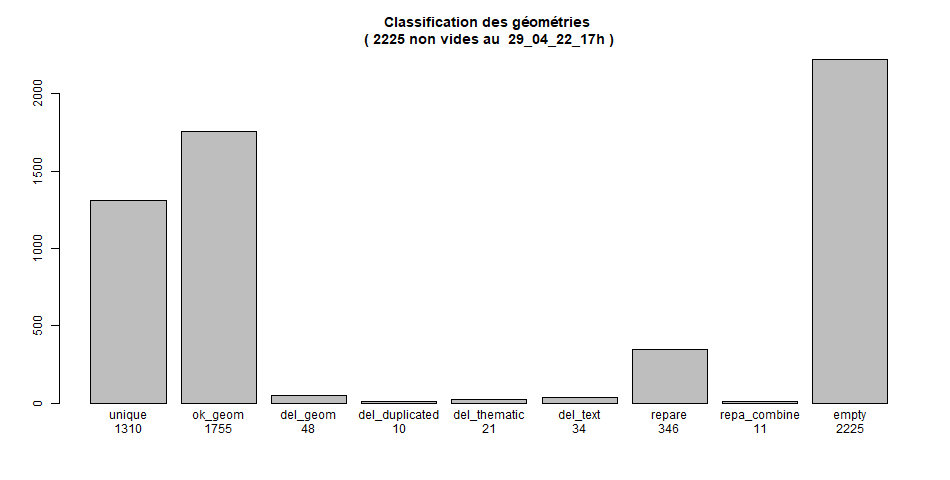
\includegraphics{./figures/bar_classify_Del_29_04_22_17h.png}

}

\caption{Chart Bar des NAS}

\end{figure}

\begin{Shaded}
\begin{Highlighting}[numbers=left,,]
\FunctionTok{library}\NormalTok{(ggplot2)}

\NormalTok{mtcars2 }\OtherTok{\textless{}{-}}\NormalTok{ mtcars}

\NormalTok{mtcars2}\SpecialCharTok{$}\NormalTok{am }\OtherTok{\textless{}{-}} \FunctionTok{factor}\NormalTok{(}
\NormalTok{  mtcars}\SpecialCharTok{$}\NormalTok{am, }
  \AttributeTok{labels =} \FunctionTok{c}\NormalTok{(}\StringTok{"automatic"}\NormalTok{, }\StringTok{"manual"}\NormalTok{))}

\FunctionTok{ggplot}\NormalTok{(mtcars2, }\FunctionTok{aes}\NormalTok{(hp, mpg, }\AttributeTok{color =}\NormalTok{ am)) }\SpecialCharTok{+}
  \FunctionTok{geom\_point}\NormalTok{() }\SpecialCharTok{+} \FunctionTok{geom\_smooth}\NormalTok{(}\AttributeTok{formula =}\NormalTok{ y }\SpecialCharTok{\textasciitilde{}}\NormalTok{ x, }
                             \AttributeTok{method =} \StringTok{"loess"}\NormalTok{) }\SpecialCharTok{+}
  \FunctionTok{theme}\NormalTok{(}\AttributeTok{legend.position =} \StringTok{"bottom"}\NormalTok{)}
\end{Highlighting}
\end{Shaded}

\begin{figure}[H]

{\centering 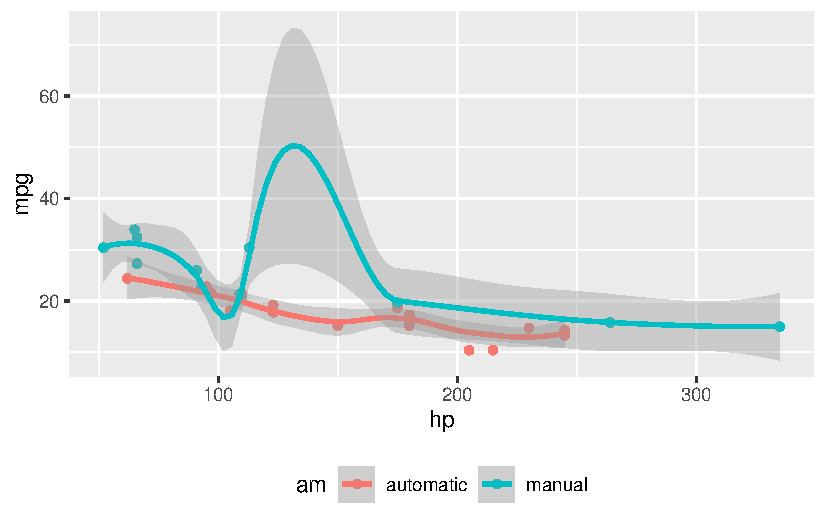
\includegraphics{./resultats_files/figure-pdf/fig-mtcars-1.pdf}

}

\caption{\label{fig-mtcars}MPG horsepower, colore by trans}

\end{figure}

Voici un graphique produir avec \texttt{R} et dot on peut lire le
(court) script

\begin{Shaded}
\begin{Highlighting}[numbers=left,,]
\FunctionTok{plot}\NormalTok{(cars)}

\FunctionTok{plot}\NormalTok{(pressure)}
\end{Highlighting}
\end{Shaded}

\begin{figure}

\begin{minipage}[t]{0.50\linewidth}

{\centering 

\raisebox{-\height}{

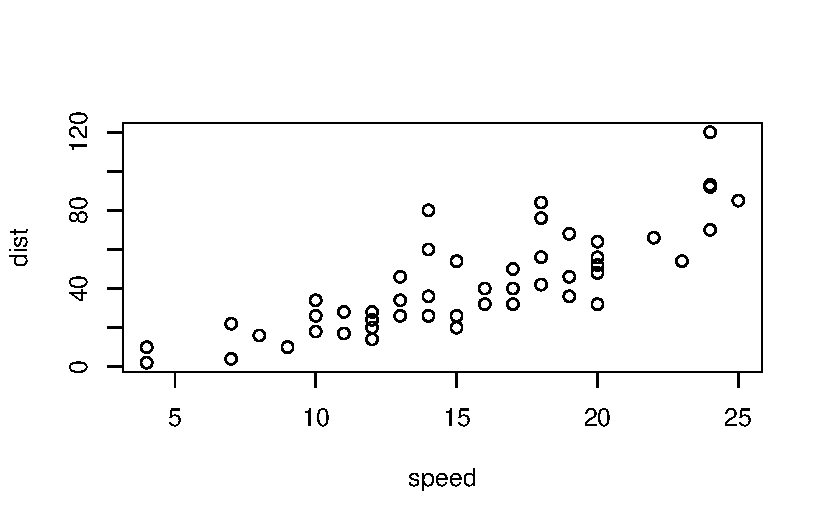
\includegraphics{./resultats_files/figure-pdf/unnamed-chunk-2-1.pdf}

}

\caption{Speed and Stopping Distances of Cars}

}

\end{minipage}%
%
\begin{minipage}[t]{0.50\linewidth}

{\centering 

\raisebox{-\height}{

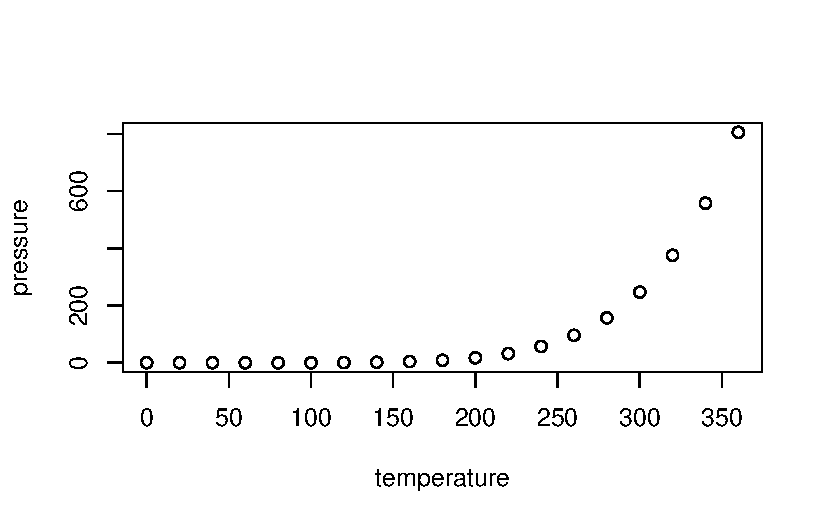
\includegraphics{./resultats_files/figure-pdf/unnamed-chunk-2-2.pdf}

}

\caption{Vapor Pressure of Mercury as a Function of Temperature}

}

\end{minipage}%

\end{figure}

\hypertarget{conclusion}{%
\chapter{Conclusion}\label{conclusion}}

Dans quelles conditions peut-on la généraliser ? Quelles réponses ont
été données ? Quelles sont celles qui ne l'ont pas été ? Que faut-il
envisager pour l'avenir ?

\hypertarget{remerciements-uxe9ventuels}{%
\chapter{Remerciements éventuels}\label{remerciements-uxe9ventuels}}

\hypertarget{references}{%
\chapter*{References}\label{references}}
\addcontentsline{toc}{chapter}{References}

\hypertarget{refs}{}
\begin{CSLReferences}{0}{0}
\end{CSLReferences}

\appendix
\addcontentsline{toc}{part}{Appendices}

\hypertarget{sec-more-results}{%
\chapter{More results}\label{sec-more-results}}

Some results that wouldn't fit into the main thesi

Some results that wouldn't fit into the main thesis

\begin{figure}

{\centering 
\includegraphics{./cover.png}

}

\caption{cover}

\end{figure}


\backmatter

\end{document}
